\chapter{Design of the Water-Skipping MAV}
\label{chapter:paperone}

\section{Design Requirements}
\label{sec:design_requirements}

The vehicle must satisfy two coupled sets of requirements: it must generate
enough lift to hover as a quadrotor, and its spinning hydrofoils must produce
sufficient hydrodynamic impulse during a brief water-surface contact to eject
it back into the air.

\paragraph{Flight requirements.}
The complete vehicle, including motion-capture markers and assembly
adhesive, has an all-up mass of $m = 90\;\mathrm{g}$.  Yaw torque is
generated by two mechanisms acting in the same rotational sense.  Two of
the four rotors are mounted horizontally, tangential to the frame, and are
driven at a fixed thrust setpoint that is set independently of the
vertical-lift channel; this direct tangential thrust is the dominant
driving torque.  The remaining two rotors are mounted vertically and
provide lift and attitude authority; because all four rotors turn in the
same physical direction, their reaction torque adds to, rather than
cancels, the tangential drive torque, contributing a secondary,
thrust-coupled term (Section~\ref{sec:mech_design}).  Because the dominant
tangential term is commanded independently of the lift channel, the
resulting spin rate is a tunable operating parameter rather than a fixed
consequence of the vehicle's thrust or airframe drag.  The attitude
controller runs at a loop rate of
$100\;\mathrm{Hz}$; a na\"ive requirement of several control updates per
revolution would place a ceiling near $\omega_z^* < 20\pi\;\mathrm{rad\,s^{-1}}$
($\approx 3600^{\circ}\,\mathrm{s^{-1}}$), but flight testing has reached
spin rates approaching $10{,}000^{\circ}\,\mathrm{s^{-1}}$ without
encountering a controllability limit.  This indicates that closed-loop
latency across the estimation, control, and actuation pipeline, not the raw number of control updates per revolution, is the more relevant constraint
on controllability at high spin rate; this relationship was not
systematically characterised in the present work and is identified as a
direction for future study (Chapter~\ref{chapter:conclusion}).  The four
rotors are driven from a $4\mathrm{S}$ high-voltage lithium polymer battery
(Coddar CD4S35090HV; \SI{15.2}{V} nominal, \SI{350}{mAh}, \SI{5.32}{Wh}, 90C
continuous discharge), supplying four Sparis \mbox{1204} motors rated at
$4{,}500\;\mathrm{KV}$.

\paragraph{Water-skipping requirements.}
For a successful hop the hydrofoils must, during the brief submersion phase,
generate a net vertical impulse large enough to reverse the vehicle's downward
velocity and return it to free flight.  Blade-element simulation of the
submersion dynamics (described in Chapter~\ref{dynamic}) shows that
both the hydrofoil inclination angle $\beta$ and the spin rate $\omega_z$
at water contact are primary drivers of the ejection velocity; the design
therefore cannot be finalised independently of the flight dynamics.

\section{Overall Mechanical Design}
\label{sec:mech_design}

% =====================================================================
% FIGURE SLOT 3.1 -- ANNOTATED VEHICLE PHOTOGRAPH  [you supply]
% Source: test results raw material/videos/photos/DSC00963.JPG (3/4 view)
% Annotate: the two tangential rotors, the two lift rotors, one hydrofoil
% leg, the Bolt board, the battery, and a mocap marker.
% To fill: delete the \fbox{...} block and uncomment the \includegraphics.
% =====================================================================
\begin{figure}[t]
    \centering
    % TODO(annotate): add callouts -- tangential rotors, lift rotors, one
    % hydrofoil leg, Bolt board, battery, mocap marker.
    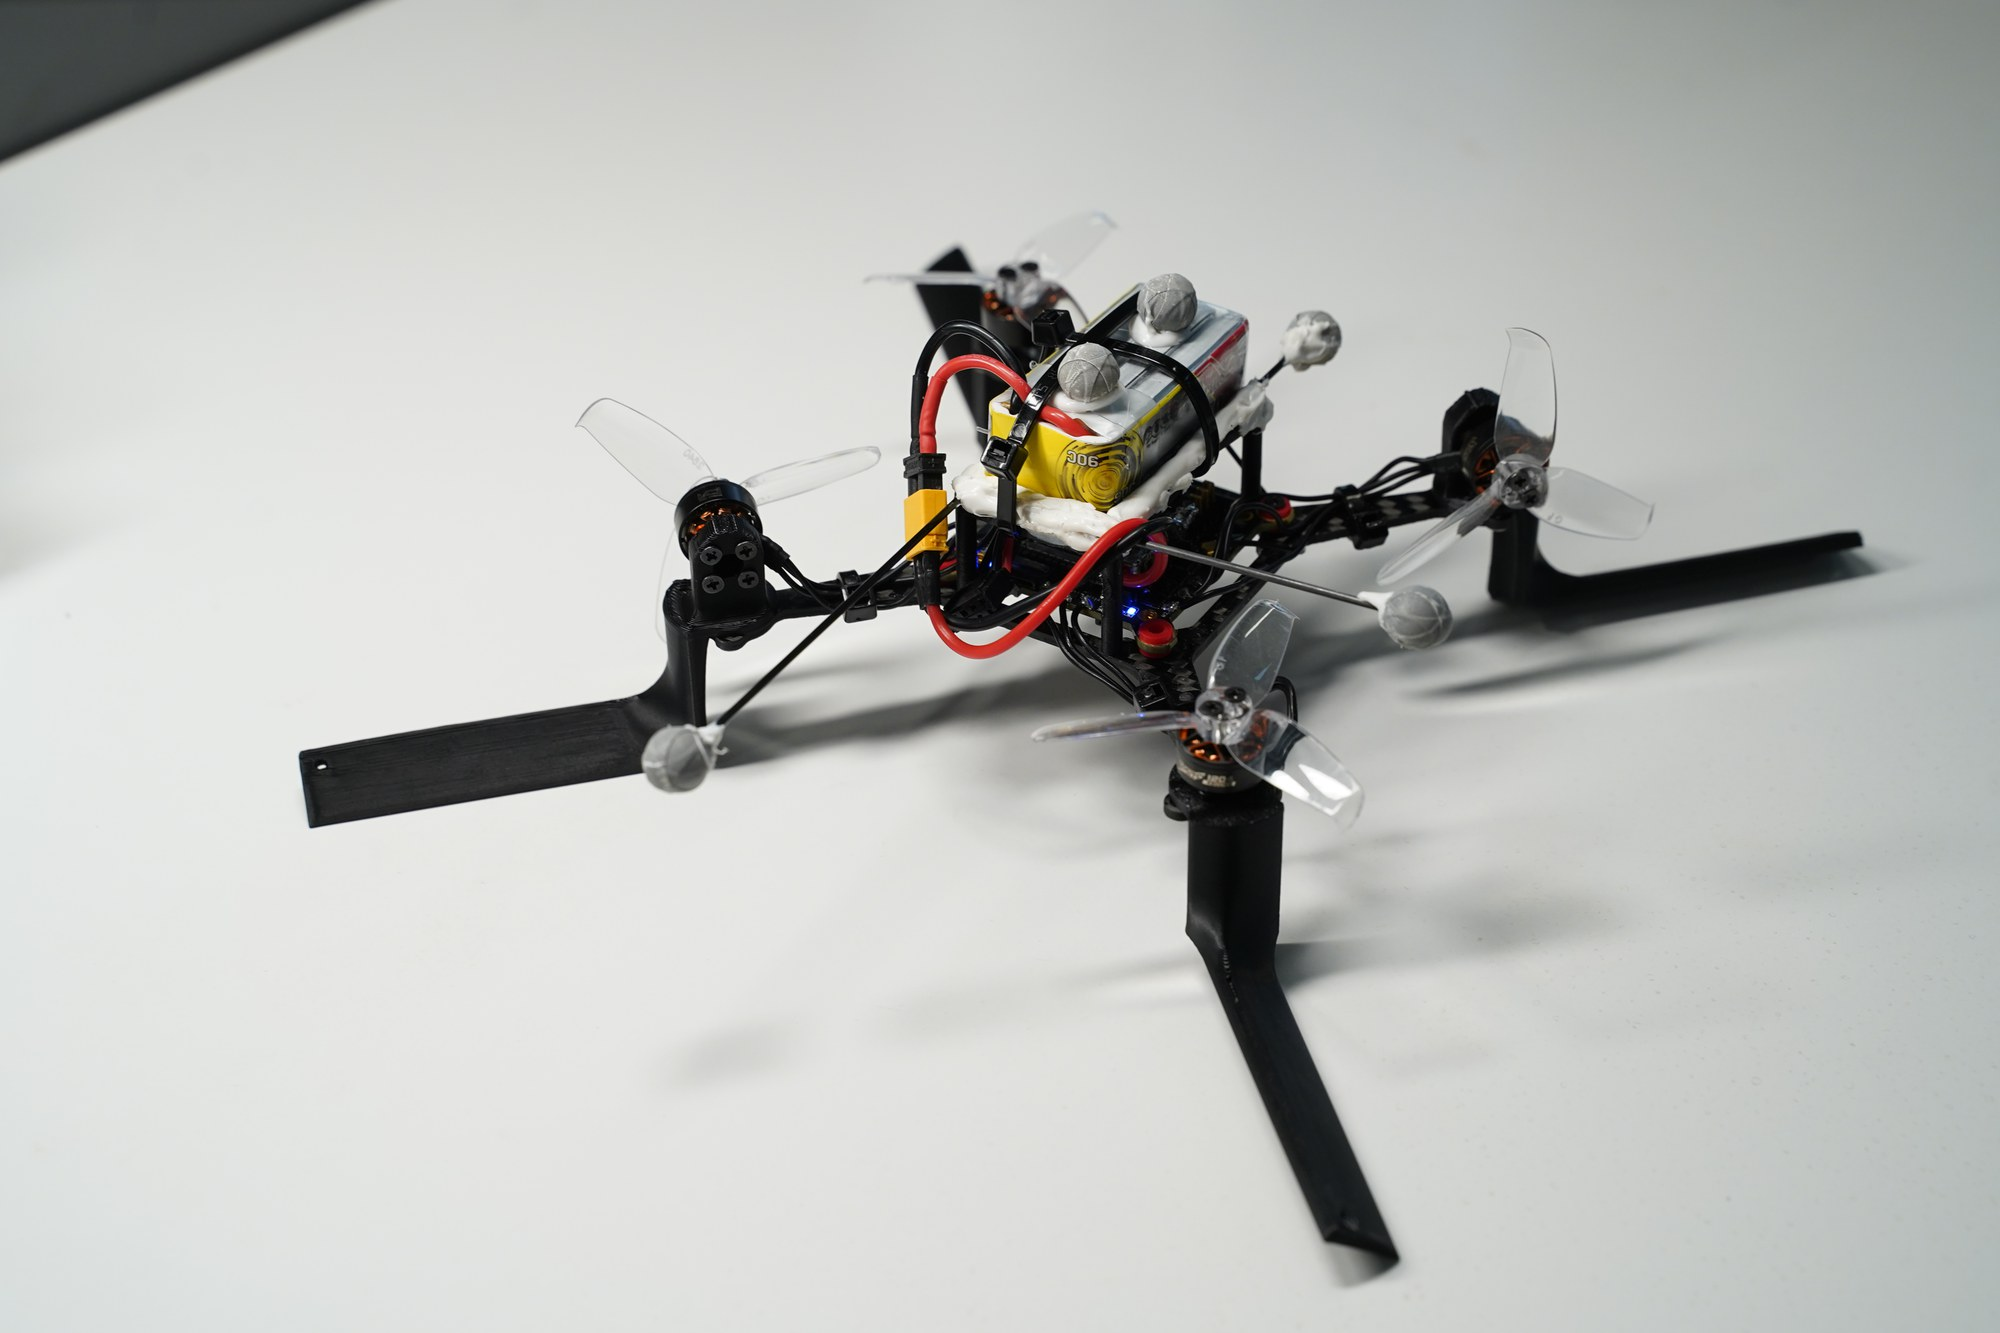
\includegraphics[width=0.85\linewidth]{Assets/ch3fig1_vehicle.jpg}
    \caption{The as-built water-skipping MAV.  Two rotors are mounted
    vertically and provide lift and attitude authority; two are mounted
    horizontally, tangential to the frame, and drive the rotation.  Each of
    the four motor mounts carries a moulded leg that drops below the airframe
    and turns outward into a hydrofoil.}
    \label{fig:vehicle_photo}
\end{figure}

\paragraph{Frame and propulsion.}
The frame carries a core of diameter $150\;\mathrm{mm}$, i.e.\ a radius of
$75\;\mathrm{mm}$ from the vehicle centre to the point where each hydrofoil
assembly begins.  Four Sparis \mbox{1204} motors, rated at
$4{,}500\;\mathrm{KV}$, are installed at this radius: two are mounted
vertically and provide lift and attitude authority, and two are mounted
horizontally, tangential to the frame, and provide yaw-drive thrust only
(Section~\ref{sec:design_requirements}).  Each motor drives a Flash
\mbox{2540-3} three-blade propeller (clear polycarbonate, T-mount).% TODO:
confirm exact azimuthal placement of the vertical vs.\ horizontal motors
for the as-built frame.

\paragraph{Electronics.}
The flight controller is a Crazyflie Bolt board, which integrates a
six-axis IMU, a radio transceiver, and motor drivers on a single compact
module.  Power is supplied by a $4\mathrm{S}$ high-voltage lithium polymer
battery (Coddar CD4S35090HV; \SI{15.2}{V} nominal, \SI{350}{mAh},
\SI{5.32}{Wh}, 90C continuous discharge).  The complete vehicle, including
motion-capture markers and assembly adhesive, has an all-up mass of
$m = 90\;\mathrm{g}$.

\paragraph{Hydrofoil mounting.}
At each of the four motor mounts, a single moulded leg drops vertically from
the frame and then kinks outward into the hydrofoil itself, so that each
hydrofoil is an integral extension of its leg rather than a separate attached part, an arrangement resembling a mosquito's legs resting on a
water surface.  The horizontal, outward-kinked span of each hydrofoil
begins at the $75\;\mathrm{mm}$ motor-mount radius and extends a further
$70\;\mathrm{mm}$, so the hydrofoil tip reaches a radius $r_f = 75 + 70 =
145\;\mathrm{mm}$ from the vehicle centre, giving an overall vehicle
diameter of $290\;\mathrm{mm}$ tip-to-tip.  The four-leg assembly rotates
with the vehicle at yaw rate $\omega_z$, as described in
Section~\ref{sec:attitude_dynamics}.

% =====================================================================
% FIGURE SLOT 3.2 -- GEOMETRY DIAGRAM  [you supply, vector/CAD]
% Two views. TOP: the 75 mm motor-mount radius, the 70 mm foil span, the
% 145 mm tip radius and the 290 mm overall diameter, with the four legs and
% the vertical/tangential rotor positions marked.
% SIDE: the leg dropping from the mount and kinking outward, showing the
% 30 deg foil inclination and the drop below the airframe.
% Base layer available: videos/photos/DSC00970.JPG (top-down, unobstructed).
% =====================================================================
\begin{figure}[t]
    \centering
    % TODO(annotate): overlay dimensions on this top-down photo -- 75 mm
    % mount radius, 70 mm foil span, 145 mm tip radius, 290 mm overall.
    % A side view still needs to be drawn and added as panel (B).
    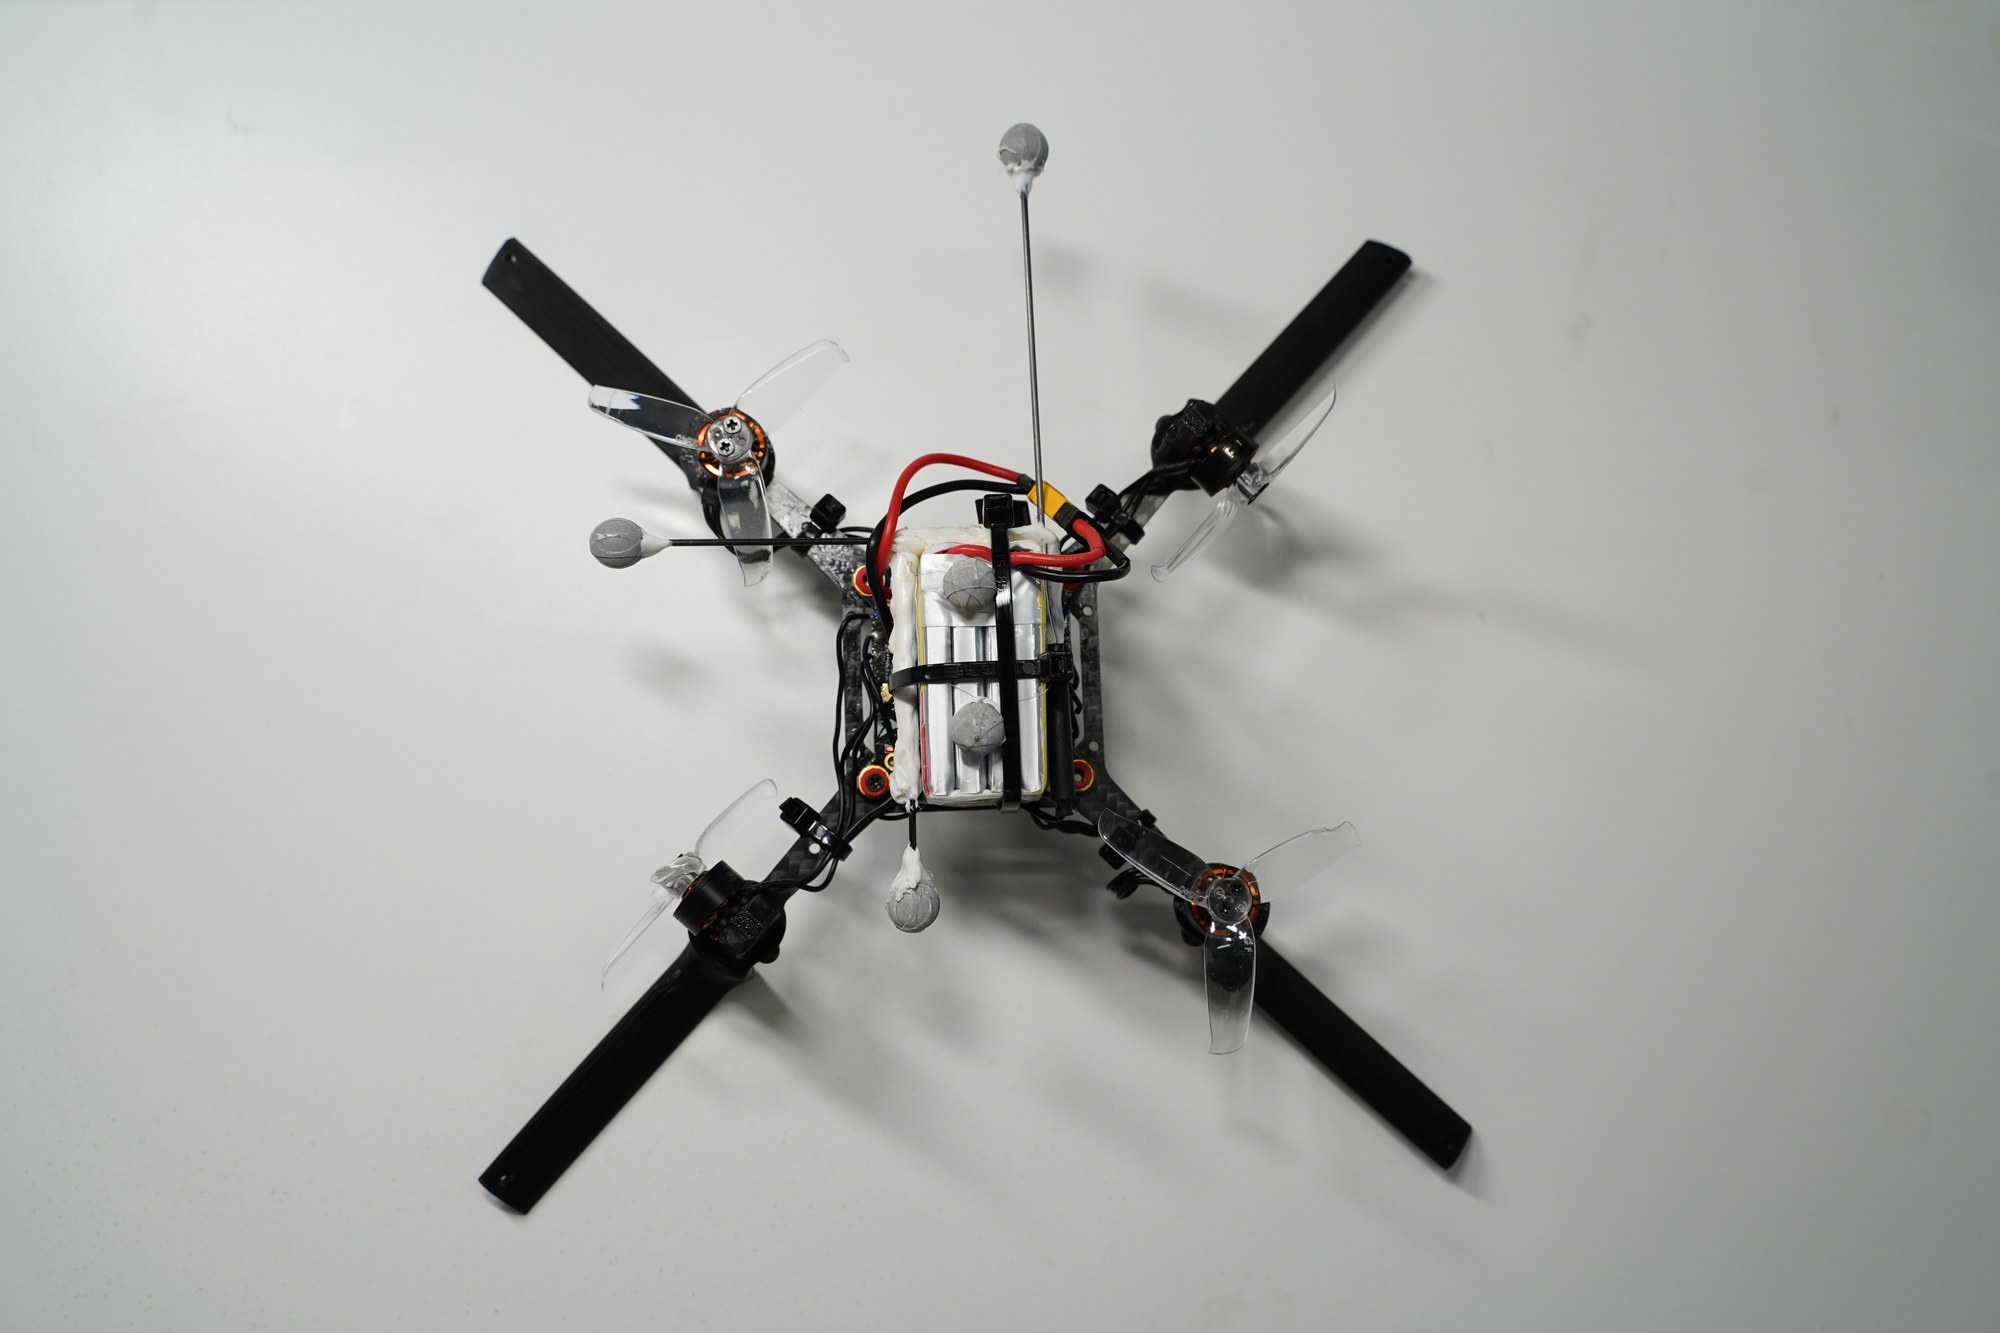
\includegraphics[width=0.85\linewidth]{Assets/ch3fig2_geometry.jpg}
    \caption{Vehicle geometry.  \textbf{(A)} Top view, showing the
    $75\;\mathrm{mm}$ motor-mount radius at which each hydrofoil begins, the
    $70\;\mathrm{mm}$ foil span, and the resulting $145\;\mathrm{mm}$ tip
    radius, giving $290\;\mathrm{mm}$ overall.  \textbf{(B)} Side view,
    showing a leg dropping from its motor mount and turning outward into the
    hydrofoil, inclined at $\beta = 30^{\circ}$ to the horizontal.}
    \label{fig:vehicle_geometry}
\end{figure}

\section{Hydrofoil Geometry}
\label{sec:foil_design}

\paragraph{Hydrofoil profile and planform.}
Each hydrofoil is a thin flat plate of thickness $3\;\mathrm{mm}$, chosen for
simplicity of fabrication and because the flat-plate hydrodynamic model
(lift coefficient $C_L = 2\sin\alpha\cos\alpha$, drag coefficient $C_D =
2\sin^2\alpha$) provides a closed-form basis for the blade-element
simulation of Chapter~\ref{dynamic}.  The foil has its own radial
length $L_f = 70\;\mathrm{mm}$, mounted with its root at the
$75\;\mathrm{mm}$ frame radius and its tip reaching $r_f = 145\;\mathrm{mm}$
from the vehicle centre (Section~\ref{sec:mech_design}), and is parametrised
by its chord $c_f$ (the dimension tangential to the sweep direction).  The
fabricated hydrofoil has chord $c_f = 15\;\mathrm{mm}$, giving a rectangular
planform area $S_f = c_f\, L_f = 1{,}050\;\mathrm{mm}^2$.

\paragraph{Attack angle.}
The hydrofoil is mounted at a fixed attack angle $\beta$ relative to the
horizontal plane, with its angled face oriented to strike the water surface
directly.  Candidate values $\beta \in \{5^{\circ}, 10^{\circ}, 15^{\circ},
20^{\circ}, 25^{\circ}, 30^{\circ}\}$ were evaluated in the blade-element
simulation of Chapter~\ref{dynamic} against predicted ejection
velocity and hop height, but only $\beta = 30^{\circ}$ was fabricated and
flight-tested; the fabricated hydrofoil is fixed at $\beta = 30^{\circ}$
with no active or passive attack-angle mechanism.  Experimental validation
of the remaining simulated angles is left to future work
(Chapter~\ref{chapter:conclusion}).

% =====================================================================
% FIGURE SLOT 3.3 -- HYDROFOIL CLOSE-UP  [you supply]
% A single leg/foil filling the frame, ideally against a plain background
% with a scale reference. Should make the 15 mm chord, the 3 mm thickness
% and the 30 deg inclination readable, and show that the leg and foil are
% one moulded part rather than an assembly.
% =====================================================================
\begin{figure}[t]
    \centering
    %\includegraphics[width=0.7\linewidth]{Assets/ch3fig3_hydrofoil.jpg}
    \fbox{\begin{minipage}[c][40mm][c]{0.7\linewidth}\centering\itshape
        Figure pending: hydrofoil close-up
    \end{minipage}}
    \caption{A single hydrofoil.  The leg and the foil are one moulded part:
    the leg drops vertically from the motor mount and turns outward into a
    flat plate of $15\;\mathrm{mm}$ chord and $3\;\mathrm{mm}$ thickness, held
    at $30^{\circ}$ to the horizontal.}
    \label{fig:hydrofoil_closeup}
\end{figure}

\section{Structural Analysis of the Hydrofoils}
\label{sec:foil_fea}

\todobox{structural analysis, or cut this section}{%
This section is a stub. Either carry out the finite-element work outlined
below, or delete the section: an empty heading is worse than no heading. For
a conference submission the argument does not depend on it, and the foils
survived every flight reported in Chapter~\ref{chapter:paperthree}, which is
itself the relevant evidence. Recommend cutting unless the analysis is
already in hand.}

% TODO: ANSYS FEA of the candidate hydrofoil geometries.
% Loads: peak water-impact distributed pressure extracted from the
%   blade-element model (Chapter~\ref{dynamic}); root clamped at mount.
% Static structural: max von Mises vs yield (safety factor); tip deflection
%   as fraction of chord (justifies the rigid-foil assumption in the BEM model).
% Modal: first natural frequencies vs spin/impact excitation.
% Geometry + material sweep -> stiffness/strength/mass trade table feeding
%   the foil-set selection in Section~\ref{sec:foil_design}.